\section{Módulos y Aplicaciones Implementadas}

Para cubrir las necesidades operativas y comerciales de \textbf{WAYKI TREK S.A.C.}, se instalaron y configuraron aplicaciones clave dentro del ecosistema de Odoo. Se han excluido de este listado los módulos de sistema por defecto (como Conversaciones, Ajustes y Aplicaciones), enfocándose únicamente en las herramientas de negocio habilitadas.

\begin{figure}[h!]
    \centering
    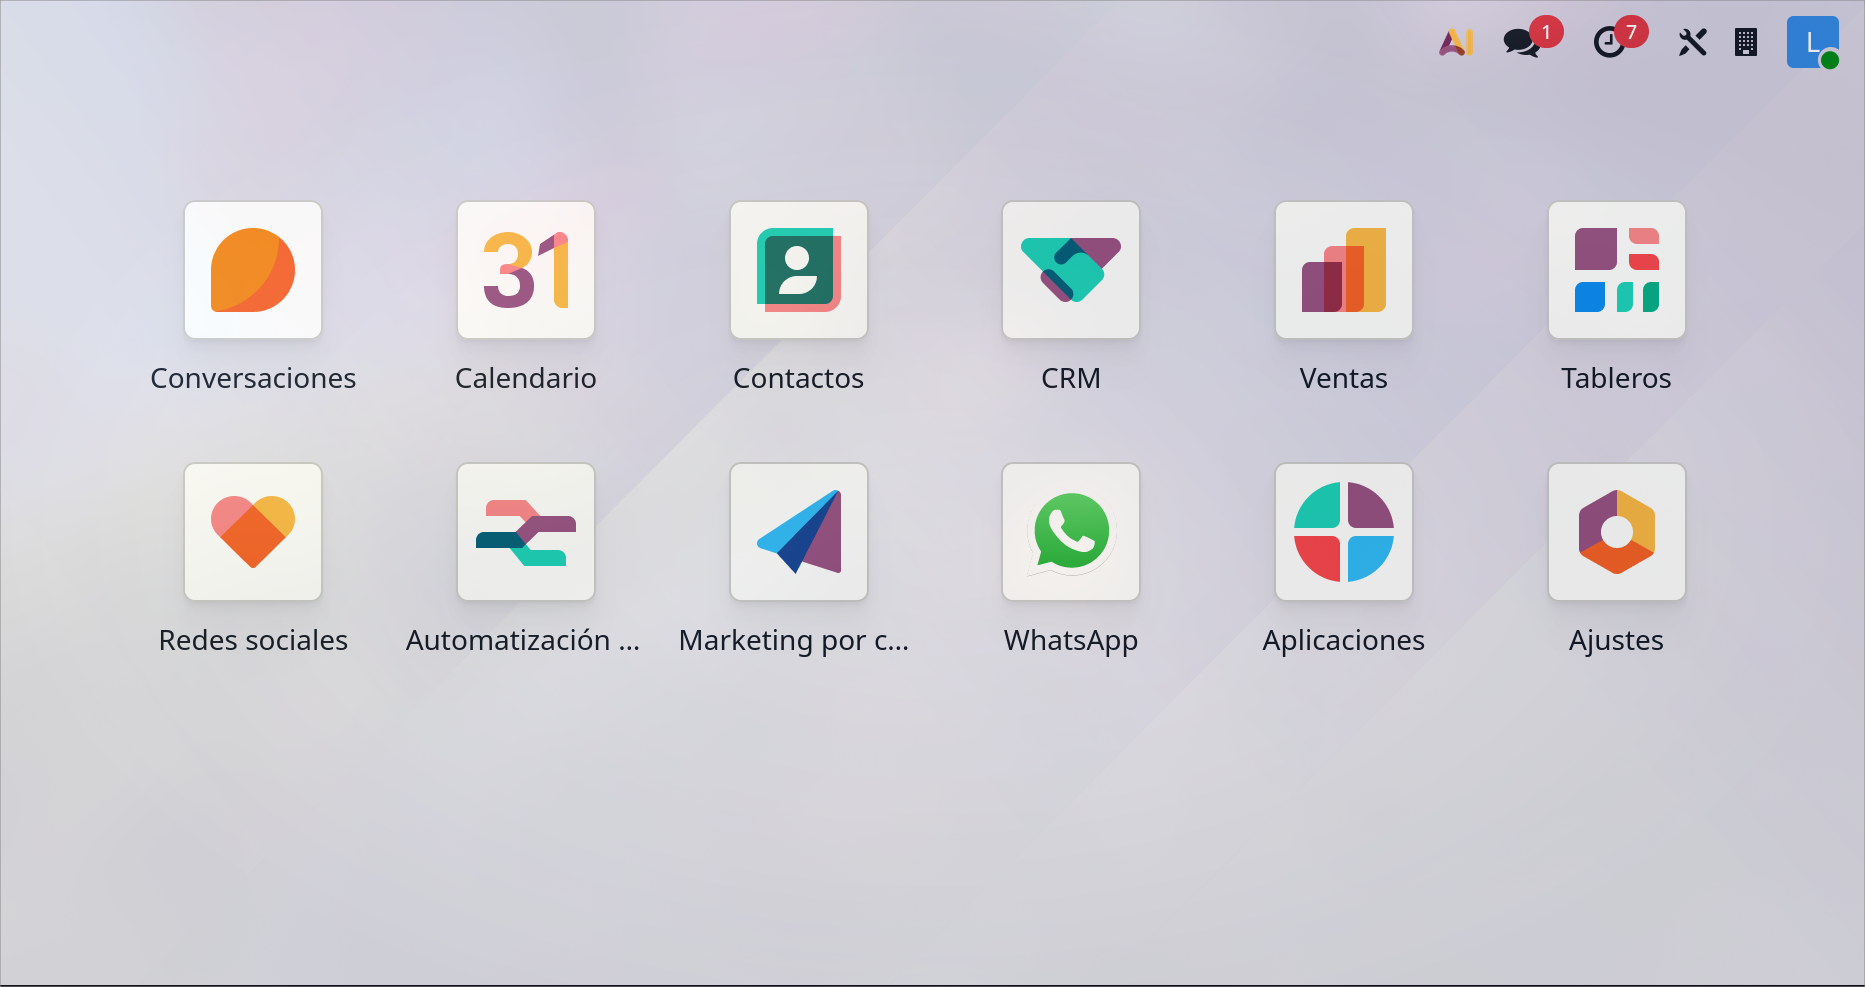
\includegraphics[width=0.9\textwidth]{assets/modulos.png}
    
    \caption{Panel principal con las aplicaciones instaladas en producción.}
    \label{fig:modulos}
\end{figure}

\subsection{Listado de Herramientas Operativas}

\begin{itemize}
    \item \textbf{CRM (Customer Relationship Management):} Eje central para el seguimiento de \textit{Leads} y oportunidades. Se configuró para gestionar el embudo de ventas y las distintas etapas de conversión de los prospectos turísticos.
    \item \textbf{Ventas:} Parametrizado para la emisión de cotizaciones/presupuestos, manejo de listas de precios y cierre formal de las reservas de los servicios.
    \item \textbf{Contactos:} Base de datos centralizada de clientes (pasajeros), agencias y proveedores, interconectada transversalmente con todos los demás módulos de la plataforma.
    \item \textbf{Calendario:} Herramienta de agenda para la gestión de citas, llamadas de seguimiento y reuniones programadas con los prospectos.
    \item \textbf{Tableros (Dashboards):} Módulo analítico que centraliza la creación de reportes visuales y KPIs de toda la operación y el rendimiento del equipo.
    \item \textbf{Marketing por Correo Electrónico:} Configurado para el envío masivo de boletines, campañas informativas y seguimiento de apertura de correos.
    \item \textbf{Automatización de Marketing:} Motor lógico para crear campañas automáticas (workflows) basadas en el comportamiento del cliente y disparadores (\textit{triggers}) específicos de tiempo o acción.
    \item \textbf{Redes Sociales:} Integración diseñada para la gestión, monitoreo y programación de publicaciones en plataformas externas.
    \item \textbf{WhatsApp:} Canal directo de mensajería integrado al flujo del CRM para brindar respuestas ágiles e interacciones oficiales con los pasajeros.
\end{itemize}

Cada uno de estos módulos ha sido parametrizado respetando la información base de la empresa y adaptando los flujos a las particularidades operativas del sector turismo que maneja Wayki Trek.
